% Versão inicial do TCC (formato artigo, modelo SBC), escrita em 2026-11-14.
% Estrutura espelhada no artigo do SBQS 2025 (docs/Critical_Failure_Artigo.pdf), por orientação.
% Compilar: pdflatex main && bibtex main && pdflatex main && pdflatex main
% Fonte de cada número: docs/RESUMO_DOS_RESULTADOS.md e os relatorio.md citados em comentários.

\documentclass[12pt]{article}

\usepackage[utf8]{inputenc}
\usepackage[T1]{fontenc}
% O babel e o hyperref vêm antes do sbc-template: na ordem inversa, o gancho de fim de preâmbulo do
% sbc-template (que ajusta a bibliografia quando há hyperref) quebra o babel com a versão de 2026 do
% LaTeX ("Undefined control sequence" em \begin{document}).
\usepackage[brazilian]{babel}
\usepackage[hidelinks]{hyperref}
\usepackage{sbc-template}
\usepackage{graphicx,url}
\usepackage{booktabs}
\usepackage{multirow}
\usepackage{array}
\usepackage{tabularx}
\usepackage[table]{xcolor}
\usepackage{tikz}
\usetikzlibrary{arrows.meta,positioning,shapes.geometric,calc}
\usepackage{pgfplots}
\pgfplotsset{compat=1.18}
\usepackage{enumitem}

% Marcador do que o autor ainda precisa completar ou revisar.
\newcommand{\pendente}[1]{\textcolor{red}{\textbf{[Pendente:} #1\textbf{]}}}

\sloppy

\title{Critical Failure 2: redesenho e verificação do balanceamento por simulação de um jogo de cartas para
o ensino de testes não funcionais}

\author{Erik Freire Ramos\inst{1}, Yuska Paola Costa Aguiar\inst{1} (orientadora)}

\address{Centro de Informática -- Universidade Federal da Paraíba (UFPB)\\
  João Pessoa -- PB -- Brasil}

\begin{document}

% Capa e folha de aprovação do Centro de Informática (UFPB).
% Substituir este arquivo pelas páginas do modelo do curso (capa, ficha catalográfica e folha de aprovação).
\pagenumbering{Alph}
\begin{titlepage}
  \centering
  {\large UNIVERSIDADE FEDERAL DA PARAÍBA\\ CENTRO DE INFORMÁTICA\\
   BACHARELADO EM CIÊNCIA DA COMPUTAÇÃO\par}
  \vspace{4cm}
  {\large Erik Freire Ramos\par}
  \vspace{2cm}
  {\Large\bfseries Critical Failure 2: redesenho e verificação do balanceamento por simulação de um jogo de
  cartas para o ensino de testes não funcionais\par}
  \vspace{3cm}
  {\normalsize Trabalho de Conclusão de Curso apresentado ao Centro de Informática da Universidade Federal da
  Paraíba, como requisito para a obtenção do grau de Bacharel em Ciência da Computação.\par}
  \vspace{1cm}
  {\normalsize Orientadora: Profa. Yuska Paola Costa Aguiar\par}
  \vfill
  {\normalsize João Pessoa\\ \pendente{mês e ano da defesa}\par}
  \vspace{1cm}
  \pendente{substituir pela capa, ficha catalográfica e folha de aprovação do modelo do CI}
\end{titlepage}
\pagenumbering{arabic}


\maketitle

\begin{abstract}
  Critical Failure is a card game for teaching non-functional testing and the quality characteristics of
  ISO/IEC 25010. Its first classroom use showed unbalanced matches: the leader tended to keep winning.
  This work redesigns the rules (version 2) and verifies their balance before new classroom sessions, treating
  balance as a set of non-functional requirements with acceptance criteria. A deterministic, auditable
  simulator played 971,000 matches between bots with different playing styles. The leader's advantage after the
  first cycle fell from about 0.40 in version 1 to about 0.09 in version 2; 10 of 13 balance requirements pass,
  and the best style mixes building and attacking. A playtest with 7 respondents reported fun and clear links to
  the course content, with the bluffing phase as the most confusing part.
\end{abstract}

\begin{resumo}
  O Critical Failure é um jogo de cartas para o ensino de testes não funcionais e das características de
  qualidade da ISO/IEC 25010. Na primeira aplicação em sala, as partidas foram desequilibradas: quem liderava
  tendia a continuar vencendo. Este trabalho redesenha as regras (versão 2) e verifica o seu balanceamento antes
  de novas aplicações, tratando o balanceamento como um conjunto de requisitos não funcionais com critério de
  aceite. Um simulador determinístico e auditável jogou 971 mil partidas entre bots com estilos diferentes.
  A vantagem de quem lidera após o primeiro ciclo caiu de cerca de 0,40 na versão 1 para cerca de 0,09 na
  versão 2; 10 de 13 requisitos de balanceamento passam, e o melhor estilo mistura construir e atacar. Um
  playtest com 7 respondentes relatou diversão e relação clara com a disciplina, com a fase de blefe como a
  parte mais confusa.
\end{resumo}

\noindent\textbf{Palavras-chave:} teste não funcional; jogos educacionais; balanceamento de jogos;
simulação; ISO/IEC 25010.

\section{Introdução}
\label{sec:introducao}

O teste de software é uma das principais atividades para garantir a qualidade e a confiabilidade de um
sistema \cite{ahamed2010}. Dentro dele, o teste não funcional, que verifica desempenho, segurança,
confiabilidade, usabilidade e outras características de qualidade, ainda recebe pouco espaço nos cursos de
graduação, apesar da sua relevância na indústria \cite{garousi2020}. Diferentemente do teste funcional, que
verifica se o sistema faz o que foi especificado, o teste não funcional avalia \emph{como} o sistema se comporta
sob diferentes condições, o que o torna mais abstrato e mais difícil de ensinar \cite{paschoal2018}. Aulas
expositivas e exercícios isolados costumam ser insuficientes para que os estudantes liguem as definições dos
livros a decisões práticas \cite{valle2015,vanhanen2018}.

Jogos educacionais vêm sendo usados para enfrentar esse problema no ensino de teste de software
\cite{costa2024debug,gomes2021gamut,beppe2018greatest,jesus2020}. Nesse contexto, a primeira versão do
\emph{Critical Failure} foi criada na disciplina de Teste de Software do Centro de Informática da UFPB
\cite{oliveira2025critical}. Nela, os jogadores montam um ``sistema'' com cartas de testes não funcionais, testam
os sistemas dos colegas e podem blefar ao se defender. Dezessete estudantes jogaram e avaliaram o jogo de forma
positiva, mas a aplicação também revelou um problema de projeto: em quatro das seis partidas observadas, o
vencedor terminou com pontuação muito acima dos demais. Quem saía na frente acumulava vantagem, e os
jogadores tendiam a atacar os mais fracos, e não o líder \cite{oliveira2025critical}. O próprio artigo sugeriu
investigar se esse comportamento vinha da inexperiência dos jogadores ou de uma falha da dinâmica do jogo.

Corrigir o balanceamento de um jogo pede muitas partidas. Com pessoas, cada partida leva quase uma hora, e
algumas dezenas de partidas não bastam para separar o efeito de uma regra do acaso, do estilo dos jogadores ou
da ordem à mesa. Este trabalho trata o jogo como um \emph{sistema sob teste}: o balanceamento é escrito como um
conjunto de requisitos não funcionais com critério de aceite, e um simulador joga milhares de partidas entre
bots para verificar esses requisitos antes de levar as regras de volta à sala de aula. Assim, o trabalho aplica
teste não funcional ao próprio jogo que ensina teste não funcional.

\subsection{Objetivo e perguntas de pesquisa}

O objetivo deste trabalho é redesenhar as regras do Critical Failure e verificar, por simulação, se a nova versão
é balanceada, comparando estilos de jogo diferentes para identificar o melhor estilo e as fraquezas das regras.
Duas perguntas de pesquisa orientam o trabalho:

\begin{itemize}
  \item \textbf{QP1:} as novas regras reduzem o desequilíbrio observado na primeira versão?
  \item \textbf{QP2:} como os estudantes avaliam a experiência com a segunda versão?
\end{itemize}

\subsection{Contribuições}

As contribuições deste trabalho são:
\begin{enumerate}
  \item a segunda versão das regras do Critical Failure (v2.2.2), alinhada à ISO/IEC 25010:2023
    \cite{iso25010}, com cada correção e cada interpretação registradas;
  \item um simulador de partidas determinístico e auditável, em que toda partida pode ser refeita e cada evento
    cita a regra que o justificou;
  \item um conjunto de 13 requisitos de balanceamento com zonas de aceite fixadas antes da medição, e a
    verificação deles em 971 mil partidas;
  \item a comparação de seis estilos de jogo e de perfis de blefe, de variantes, da retirada de cada mudança
    de regra (ablação) e da sensibilidade dos parâmetros;
  \item a avaliação de um playtest com estudantes, ligada aos resultados do simulador.
\end{enumerate}

\subsection{Organização do texto}

A Seção~\ref{sec:relacionados} apresenta os trabalhos relacionados. A Seção~\ref{sec:metodologia} descreve a
metodologia, baseada em \emph{Design Science Research}. A Seção~\ref{sec:implementacao} apresenta as regras da
segunda versão e o simulador. A Seção~\ref{sec:resultados} traz os resultados, as lições aprendidas e as
limitações. A Seção~\ref{sec:conclusoes} conclui o trabalho e aponta trabalhos futuros.

\section{Trabalhos Relacionados}
\label{sec:relacionados}

Os trabalhos relacionados se dividem em três grupos: jogos para o ensino de teste de software, jogos
educacionais desenvolvidos e avaliados em trabalhos de conclusão de curso da UFPB, e o uso de agentes
artificiais para avaliar e balancear jogos.

\subsection{Jogos para o ensino de teste de software}

O \emph{Debug} é um jogo de cartas cooperativo, criado numa disciplina de graduação, para explorar níveis e
tipos de teste de software \cite{costa2024debug}. O \emph{GAMUT} usa uma narrativa de fantasia medieval para
ensinar teste de unidade \cite{gomes2021gamut}. No \emph{GreaTest}, os jogadores assumem o papel de analistas de
teste e escolhem o tipo de teste adequado a cada cenário \cite{beppe2018greatest}. O \emph{Sojourner under
Sabotage} é um jogo sério no navegador em que o jogador corrige componentes sabotados de uma nave usando teste
de unidade e depuração \cite{straubinger2025sojourner}. O \emph{JADE} é um jogo de tabuleiro para ensinar
ergonomia de software \cite{jeandaubias2023jade}. Experiências com gamificação contínua em disciplinas de teste
também mostram ganho de engajamento \cite{straubinger2024ci,jesus2020,blanco2023}.

A primeira versão do Critical Failure \cite{oliveira2025critical} ocupou uma lacuna desses trabalhos, voltados
principalmente ao teste funcional: é um jogo de cartas competitivo sobre teste não funcional e atributos de
qualidade. Os jogos citados foram avaliados pela percepção dos estudantes. Nenhum deles relata uma verificação
sistemática do equilíbrio entre os jogadores antes da aplicação em sala.

\subsection{Jogos educacionais em trabalhos de conclusão de curso da UFPB}

No repositório institucional da UFPB há trabalhos de conclusão de curso que desenvolvem jogos de cartas para o
ensino de computação: o \emph{Computer Cards}, sobre arquitetura de computadores no ensino fundamental
\cite{oliveira2022computercards}; o \emph{BI-NA-RI-OH}, sobre aritmética binária \cite{soares2023binarioh}; e o
\emph{Logic Challenge}, sobre lógica \cite{abreu2021logic}. Outro trabalho avalia um jogo de tabuleiro para o
ensino de redes de computadores com o modelo MEEGA+ \cite{martins2020redes,petri2017meega}. No Centro de
Informática, um trabalho aplicou testes automatizados a um jogo sério, o GiroJampa, com testes de unidade e
medição de cobertura \cite{ramos2023girojampa}. Nenhum desses trabalhos trata de jogo para o ensino de teste de
software nem de balanceamento verificado por simulação.

\subsection{Balanceamento e playtesting com agentes}

O uso de agentes artificiais para avaliar o projeto de jogos tem uma linha de pesquisa própria.
Jaffe et al., por exemplo, mediram o balanceamento de jogos competitivos comparando a força de
jogadores com restrições impostas, numa abordagem chamada \emph{restricted play} \cite{jaffe2012}.
Silva et al. usaram agentes com heurísticas diferentes para jogar grandes quantidades de partidas
de um jogo de tabuleiro moderno e encontrar problemas de projeto, como estratégias que dominam e situações não
previstas pelas regras \cite{silva2017ttr}. Volz et al. mostraram que é possível balancear
automaticamente o baralho de um jogo de cartas com algoritmos evolutivos e simulação \cite{volz2016}.
Holmgård et al. propuseram \emph{personas} procedurais, agentes com estilos de jogo distintos, para
testar automaticamente os níveis de um jogo \cite{holmgard2019}.

Este trabalho se apoia nessa linha, com três diferenças. Primeiro, o jogo é educacional, e parte das decisões do
jogador depende de conhecimento sobre o conteúdo, como explicar um teste ou diagnosticar um incidente. Por isso
o simulador modela o conhecimento do estudante como probabilidade de acerto. Segundo, o balanceamento é
escrito como requisitos com critério de aceite fixado antes da medição, como em um teste de aceitação. Terceiro,
o próprio simulador é verificado com técnicas de teste de software, como testes metamórficos, testes baseados
em propriedades e teste de mutação. A Tabela~\ref{tab:relacionados} resume a comparação.

\begin{table}[ht]
  \centering
  \caption{Comparação entre os trabalhos relacionados e este trabalho}
  \label{tab:relacionados}
  \small
  \begin{tabularx}{\linewidth}{>{\raggedright\arraybackslash}p{3.9cm} >{\raggedright\arraybackslash}p{2.2cm}
      >{\raggedright\arraybackslash}p{1.9cm} >{\raggedright\arraybackslash}X >{\raggedright\arraybackslash}p{2.5cm}}
    \toprule
    Trabalho & Tipo & Modo & Escopo & Balanceamento verificado \\
    \midrule
    Debug \cite{costa2024debug} & Analógico (cartas) & Cooperativo & Níveis e tipos de teste & Não \\
    GAMUT \cite{gomes2021gamut} & Digital (narrativa web) & Individual & Teste de unidade & Não \\
    GreaTest \cite{beppe2018greatest} & Analógico (cartas) & Competitivo & Teste funcional em geral & Não \\
    Sojourner under Sabotage \cite{straubinger2025sojourner} & Digital (jogo sério) & Individual & Teste de unidade e depuração & Não \\
    JADE \cite{jeandaubias2023jade} & Analógico (tabuleiro) & Cooperativo & Ergonomia de software & Não \\
    Critical Failure v1 \cite{oliveira2025critical} & Analógico (cartas) & Competitivo & Teste não funcional e atributos de qualidade & Por observação (6 partidas) \\
    Agentes para balanceamento \cite{jaffe2012} \cite{silva2017ttr} \cite{volz2016} & Jogos de entretenimento & Competitivo & Projeto de jogos & Por simulação \\
    \textbf{Este trabalho} & Analógico (cartas) e simulador & Competitivo & Teste não funcional (ISO/IEC 25010:2023) & Por simulação, com requisitos e critério de aceite \\
    \bottomrule
  \end{tabularx}
\end{table}

\section{Metodologia}
\label{sec:metodologia}

O trabalho segue a abordagem de \emph{Design Science Research} (DSR), em que artefatos são projetados para
resolver um problema prático e avaliados em ciclos iterativos \cite{hevner2004,wieringa2014}. Os artefatos são as
regras da segunda versão do Critical Failure e o simulador de partidas. Cada ciclo tem três etapas
(Figura~\ref{fig:ciclo}): as regras são redesenhadas; o simulador verifica o balanceamento com milhares de
partidas entre bots; e as regras verificadas vão para pessoas, em playtests e aplicações em sala. O que cada
etapa encontra volta para ajustar as regras.

\begin{figure}[ht]
  \centering
  % Ciclo de Design Science Research do trabalho: regras -> simulador -> pessoas -> regras.
\begin{tikzpicture}[
    etapa/.style={draw, rounded corners, thick, align=center, minimum width=3.6cm, minimum height=1.4cm,
      font=\small},
    seta/.style={-{Stealth[length=3mm]}, thick},
    rotulo/.style={font=\footnotesize, align=center}
  ]
  \node[etapa, fill=blue!8] (regras) at (0,0) {\textbf{1. Regras}\\v2.2 $\rightarrow$ v2.2.1 $\rightarrow$ v2.2.2};
  \node[etapa, fill=orange!10] (simulador) at (7.8,0) {\textbf{2. Simulador}\\971 mil partidas entre bots};
  \node[etapa, fill=green!8] (pessoas) at (3.9,-3.2) {\textbf{3. Pessoas}\\playtest e aplicação em sala};
  \draw[seta] (regras) -- node[above, rotulo] {requisitos com\\critério de aceite} (simulador);
  \draw[seta] (simulador) -- node[right, rotulo, xshift=2mm] {regras\\verificadas} (pessoas);
  \draw[seta] (pessoas) -- node[left, rotulo, xshift=-2mm] {percepções\\e tempos reais} (regras);
  \draw[seta, dashed] (simulador.north) to[bend right=25] node[above, rotulo] {correções (COR) e ajustes} (regras.north);
\end{tikzpicture}

  \caption{Ciclo de Design Science Research do trabalho}
  \label{fig:ciclo}
\end{figure}

A ordem real das etapas neste trabalho foi a seguinte. As versões 2.0, 2.1 e 2.2 das regras foram projetadas a
partir dos problemas da primeira versão. A versão 2.2 foi jogada num playtest com estudantes, entre outubro e
novembro de 2026. Em seguida, o simulador foi construído e verificou a versão 2.2. Ele levou a duas correções
(versão 2.2.1) e, depois dos experimentos, a uma recomendação de número de jogadores (versão 2.2.2).

\subsection{Redesenho das regras}

O ponto de partida foi a primeira versão (v1), descrita no artigo do SBQS 2025 \cite{oliveira2025critical}. A
v1 deixou quatro problemas:
\begin{itemize}
  \item partidas desequilibradas, em que o líder acumulava vantagem;
  \item jogadores atacando os mais fracos, e não o líder;
  \item regras confusas para quem jogava pela primeira vez, sobretudo a diferença entre as cartas do sistema e
    as da mão, e a pontuação;
  \item inconsistências na tabela de cartas publicada, como testes de Desempenho listados em Usabilidade e a
    categoria Compatibilidade com 6 cartas em vez de 9.
\end{itemize}

As versões 2.0 a 2.2 reorganizaram o jogo em ciclos de Planejamento, Homologação e Produção. A Seção~\ref{sec:implementacao}
descreve as regras. As mudanças principais da 2.1 em relação à 2.0 foram:
\begin{itemize}
  \item a classificação passou para as categorias da ISO/IEC 25010:2023 \cite{iso25010};
  \item o baralho passou para 63 cartas e 29 testes;
  \item o placar passou a ser feito em fichas;
  \item o alvo na Homologação ficou livre, sem limite de testes;
  \item foi proibido testar a mesma categoria de um jogador que já tem Alerta nela (o ``bug duplicado'');
  \item o Hotfix foi retirado.
\end{itemize}
A 2.2 reescreveu os incidentes: a frente traz só o relato, e o verso, o gabarito.

Durante a especificação do simulador, cada regra virou um item numerado (por exemplo, R-7.3.4). Cada ponto
ambíguo ou omisso virou uma entrada de um registro de ambiguidades: foram 30, 10 delas da v1, todas decididas pelo autor. Três
decisões mudaram as regras e geraram novas versões, cada uma com o seu arquivo de texto e o seu arquivo de
configuração:
\begin{itemize}
  \item \textbf{COR-01:} máximo de 5 jogadores, em vez de 6, porque com 6 a preparação e os três Planejamentos
    pedem 71 cartas, e o baralho tem 63;
  \item \textbf{COR-02:} todos os Alertas saem no início de cada Planejamento;
  \item \textbf{COR-03:} 4 jogadores como número recomendado, depois dos experimentos (Seção~\ref{sec:resultados}).
\end{itemize}
Toda correção fica atrás de uma chave de configuração, de modo que a regra impressa continua disponível para medir
o efeito da mudança.

\subsection{O simulador como sistema sob teste}

O simulador trata o jogo como um sistema sob teste. Os bots fazem o papel de usuários virtuais, como num teste de
carga, e o balanceamento é escrito como requisitos não funcionais com critério de aceite. A
Tabela~\ref{tab:requisitos} lista os 13 requisitos. A medida e a zona de aceite de cada um foram confirmadas pelo
autor antes do primeiro experimento que o mede, para que o critério não fosse escolhido depois de ver o
resultado.

\begin{table}[ht]
  \centering
  \caption{Requisitos de balanceamento e zonas de aceite}
  \label{tab:requisitos}
  \footnotesize
  \begin{tabularx}{\linewidth}{>{\raggedright\arraybackslash}p{3.1cm} >{\raggedright\arraybackslash}X
      >{\raggedright\arraybackslash}p{3.3cm}}
    \toprule
    Requisito & Medida & Zona de aceite \\
    \midrule
    REQ-01 Equidade de assento & Taxa de vitória de cada posição na ordem, com bots iguais & $1/N \pm 0{,}02$ \\
    REQ-02 Anti bola de neve & Vantagem do líder: chance de vencer de quem lidera sozinho no fim do ciclo~1, menos $1/N$ & v2 menor que a v1 por $\geq 0{,}05$ \\
    REQ-03 Habilidade importa & Vitória do bot Heurístico contra bots Aleatórios & acima de $1{,}5/N$ \\
    REQ-04 Sem estratégia dominante & Nenhum estilo ou perfil de blefe é a melhor resposta contra todas as mesas & nenhum dominante \\
    REQ-05 Blefes bem-sucedidos & Blefes que terminam sem Alerta, sobre blefes tentados, no equilíbrio & 0,30 a 0,50 \\
    REQ-06 Distribuição de ataques & (a) máximo sobre a média de testes recebidos; (b) fração dos testes contra o menor placar & (a) até 1,5; (b) até $\frac{1}{N-1}+0{,}10$ \\
    REQ-07 Fichas não zeram cedo & Partidas com alguém em 0 ficha antes do ciclo~3 & até 0,10 \\
    REQ-08 Duração & Mediana da duração estimada pelo modelo de tempos & 40 a 50 min \\
    REQ-09 Robustez & Exceções e violações de invariantes & 0 em $\geq 50.000$ partidas \\
    REQ-10 Tempo parado & Percentil 90 do tempo parado por jogador e ciclo & abaixo de 5 min \\
    REQ-11 Os dois estilos aparecem & Jogadores com o sistema cheio no fim do 1º Planejamento & 0,10 a 0,90 \\
    REQ-12 O 1º incidente não decide & Diferença de vitória entre quem começa cobrindo o incidente~1 e os demais & até 0,10 \\
    REQ-13 Incidentes pesam & Fichas movimentadas pelos incidentes (dano e diagnóstico) sobre o total & 0,20 a 0,60 \\
    \bottomrule
  \end{tabularx}
\end{table}

Cada medida é estimada com intervalo de confiança de 95\%: o de Wilson para proporções \cite{wilson1927} e o
\emph{bootstrap} para razões e quantis \cite{efron1993}. O veredito segue uma regra fixa:
\begin{itemize}
  \item \textbf{passa} quando o intervalo inteiro está dentro da zona;
  \item \textbf{falha} quando o intervalo inteiro está fora da zona;
  \item \textbf{inconclusivo} quando o intervalo cruza a borda.
\end{itemize}
Com uma zona de aceite, uma diferença mínima e sem importância prática não reprova um requisito só porque o
número de partidas é grande. Os requisitos que dependem do comportamento dos bots, como o blefe e a ausência de
estratégia dominante, são avaliados com uma matriz de ganhos entre perfis e com a dinâmica do replicador
\cite{taylor1978}, que aponta o equilíbrio para onde uma população de jogadores tenderia.

Toda partida é reproduzível. A aleatoriedade deriva de uma semente mestre, do número da partida e de um
contador, o estado do motor não usa ponto flutuante, e a mesma semente gera o mesmo registro em qualquer
plataforma. Toda partida pode gerar um registro de auditoria, em que cada evento separa a informação pública da
oculta, cita a regra que o justificou e traz o resumo criptográfico do estado. Cada experimento oficial só roda
com o código registrado no git e grava um manifesto com o commit, as configurações e a semente. Assim, cada
número deste texto pode ser refeito.

A Tabela~\ref{tab:experimentos} lista os experimentos. Ao todo, foram 13 execuções oficiais e 971 mil partidas,
sem nenhuma falha. A v1 também foi implementada, mas só para ser observada e comparada, nunca ajustada.

\begin{table}[ht]
  \centering
  \caption{Experimentos com o simulador}
  \label{tab:experimentos}
  \footnotesize
  \begin{tabularx}{\linewidth}{>{\raggedright\arraybackslash}p{3.6cm} >{\raggedright\arraybackslash}X r}
    \toprule
    Experimento & Pergunta & Partidas \\
    \midrule
    Linha de base & Equidade de assento, duração e robustez, com bots aleatórios & 90.000 \\
    Fumaça dos estilos & Os estilos de bot jogam de forma diferente? & 20.000 \\
    1. Validação da v1 & A v1 simulada mostra o desequilíbrio do artigo? & 85.000 \\
    2. v1 $\times$ v2.2.1 & A v2 reduz a vantagem do líder? (QP1) & 40.000 \\
    Melhor estilo & Matriz de 6 estilos, com 4 e 5 jogadores & 140.000 \\
    5 e 5b. Equilíbrio do blefe & Torneio entre 9 perfis puros de blefe e mesa do equilíbrio & 200.000 \\
    6. Variantes & 9 variantes propostas para o playtest, uma de cada vez (repetido com o REQ-13 redefinido) & 160.000 \\
    3. Ablação & O que acontece ao desfazer cada mudança da 2.2? & 36.000 \\
    4 e 4b. Sensibilidade & Fichas iniciais, dano dos incidentes, tempos e combinações & 120.000 \\
    7. Profundidade & Testes sem limite contra limites e custo por teste & 80.000 \\
    \midrule
    \textbf{Total} & & \textbf{971.000} \\
    \bottomrule
  \end{tabularx}
\end{table}

\subsection{Playtest com estudantes}

A versão 2.2, com o módulo opcional de Segurança Operacional, foi jogada por cerca de 30 estudantes
\pendente{confirmar o número de participantes, a turma e as datas das sessões}. Depois da partida, os
participantes responderam a um questionário online, anônimo e com termo de consentimento; 7 responderam, entre
19 de outubro e 3 de novembro de 2026. O questionário tinha:
\begin{itemize}
  \item perguntas de perfil (curso, período, experiência com teste, frequência com jogos de mesa e
    conhecimento prévio);
  \item 11 afirmações baseadas nas dimensões do modelo MEEGA+ \cite{petri2017meega}, numa escala de 5 pontos;
  \item 4 afirmações sobre a contribuição percebida para a aprendizagem e 6 sobre as regras;
  \item a duração percebida, a parte mais confusa das regras e as impressões sobre a experiência;
  \item 3 perguntas abertas.
\end{itemize}
As respostas são analisadas de forma descritiva. Elas não são publicadas, para proteger os participantes, e só
as contagens agregadas aparecem neste texto.

\section{Implementação}
\label{sec:implementacao}

\subsection{A ideia e a caracterização}

Na segunda versão, cada jogador lidera uma equipe que constrói um sistema de software e, ao mesmo tempo, testa
o sistema dos colegas. O sistema é posto à prova de duas formas: pelos colegas, na Homologação, e pelo ``mundo
real'', na Produção, em que incidentes atingem todos ao mesmo tempo. O blefe continua no centro do jogo: quem é
testado pode afirmar que tem o teste certo e explicá-lo com as próprias palavras, tendo ou não a carta. Um
Auditor, que muda a cada ciclo, confere a explicação. Vence quem terminar com mais Fichas de Reputação. A
Tabela~\ref{tab:visao-geral} resume o jogo.

\begin{table}[ht]
  \centering
  \caption{Visão geral do Critical Failure 2.2.2}
  \label{tab:visao-geral}
  \small
  \begin{tabular}{>{\raggedright\arraybackslash}p{4.2cm} >{\raggedright\arraybackslash}p{9cm}}
    \toprule
    Nome & Critical Failure 2.2.2 \\
    Tipo & Competitivo, com blefe e dedução \\
    Escopo & Testes não funcionais; 7 características de qualidade da ISO/IEC 25010:2023 \\
    Jogadores & 4 a 5 (recomendado: 4) \\
    Cartas de Teste & 63 (9 por categoria, 29 testes); 72 e 33 testes com o módulo \\
    Cartas de Incidente & 14 (2 por categoria); 16 com o módulo \\
    Estrutura & 3 ciclos (Planejamento, Homologação, Produção), Critical Failure e revelação \\
    Duração estimada & 40 a 50 minutos (a validar no playtest) \\
    \bottomrule
  \end{tabular}
\end{table}

\subsection{As cartas do jogo}

Cada categoria do jogo é um tipo de teste não funcional e corresponde a uma característica de qualidade da
ISO/IEC 25010:2023 \cite{iso25010}. Adequação Funcional, a nona característica da norma, fica de fora por ser
funcional. A Segurança Operacional (\emph{safety}) entra como módulo opcional. Em relação à v1, Usabilidade passa
a se chamar Interação, Portabilidade passa a ser Flexibilidade, Segurança passa a ser Segurança da Informação,
Escalabilidade sai de Desempenho e vai para Flexibilidade, e Manutenibilidade entra como categoria nova.

As Cartas de Teste trazem só a categoria e o nome do teste. A descrição de cada teste e a lista do que não deve
ser confundido com ele ficam no Documento do Auditor. Assim, o jogador precisa explicar o teste com as próprias
palavras. A Tabela~\ref{tab:cartas} mostra o baralho do jogo base.

\begin{table}[ht]
  \centering
  \caption{Cartas de Teste do jogo base (cópias de cada teste entre parênteses)}
  \label{tab:cartas}
  \footnotesize
  \begin{tabularx}{\linewidth}{>{\raggedright\arraybackslash}p{3.3cm} >{\raggedright\arraybackslash}X c}
    \toprule
    Categoria & Testes & Cartas \\
    \midrule
    Desempenho & Carga (3), Estresse (2), Pico (2), Resistência (2) & 9 \\
    Compatibilidade & Coexistência (3), Interoperabilidade (2), Contrato de API (2), Retrocompatibilidade (2) & 9 \\
    Interação & Acessibilidade (3), Proteção contra erro do usuário (2), Teste A/B (2), Teste com usuários (2) & 9 \\
    Confiabilidade & Recuperação (3), Tolerância a falhas (2), Disponibilidade (2), Engenharia do Caos (2) & 9 \\
    Segurança da Informação & Autenticação (2), Confidencialidade (2), Integridade (2), Não repúdio (1), Penetração (2) & 9 \\
    Manutenibilidade & Regressão (3), Análise estática (2), Revisão de código (2), Análise de impacto (2) & 9 \\
    Flexibilidade & Escalabilidade (3), Adaptabilidade (2), Instalabilidade (2), Substituibilidade (2) & 9 \\
    \midrule
    \textbf{Total} & 29 testes & \textbf{63} \\
    \bottomrule
  \end{tabularx}
\end{table}

As Cartas de Incidente têm duas faces. A frente traz o relato de um problema, com o sintoma e a evidência, e fica
visível desde que a carta entra no Radar de Riscos. O verso é o gabarito: a categoria-chave, uma categoria
secundária opcional, um ou dois testes-chave, a explicação e o dano. Há dois incidentes por categoria, e três
deles são severos. Por exemplo, o relato do incidente ``Abertura da venda de ingressos'' diz que o site ficou 15
minutos sem responder quando 50 mil pessoas entraram no mesmo segundo, e que tudo voltou ao normal sozinho, com
os mesmos servidores. A categoria-chave é Desempenho, os testes-chave são Pico e Estresse, e Confiabilidade
aparece como secundária.

\subsection{As regras do jogo}

\textbf{Preparação.} Cada jogador recebe 5 fichas e 2 Cartas de Teste sorteadas, viradas para baixo, que formam o
seu sistema inicial. Três incidentes e a carta Critical Failure formam a Linha do Tempo. O Radar de Riscos mostra
o relato do incidente do ciclo (vaga Agora) e o do próximo (vaga Próximo). Cinco cartas viradas para cima formam
o Backlog.

\textbf{Planejamento.} Na sua vez, cada jogador compra 3 cartas, do Backlog ou do baralho, e coloca no sistema
quantas quiser, até o teto de 5 cartas, sem troca. Toda carta que não vai para o sistema é munição para testar os
colegas. Essa é a principal decisão de gestão do jogo: encher o sistema protege contra os incidentes, mas tira
munição e engessa o sistema.

\textbf{Homologação.} Na sua vez, o jogador testa qualquer colega ou passa. O atacante joga uma carta e anuncia o
teste e a categoria. O defensor admite a falha ou nomeia um teste daquela categoria que diz ter no sistema e o
explica com as próprias palavras, tendo ou não a carta. O Auditor compara a explicação com o Documento do
Auditor. Se a explicação conferir, o atacante aceita ou contesta. Os resultados são:
\begin{itemize}
  \item \textbf{falhou} (o defensor admitiu ou a explicação não conferiu): o atacante ganha 1 ficha, e o defensor
    recebe um Alerta na categoria;
  \item \textbf{defesa aceita}: nada acontece;
  \item \textbf{contestou, e o defensor tinha a carta}: o atacante paga 1 ficha ao defensor;
  \item \textbf{contestou, e era blefe}: o defensor paga 1 ficha ao atacante, o atacante ganha mais 1 do banco, e o
    defensor recebe Alerta.
\end{itemize}
Não há limite de testes, mas é proibido testar um jogador numa categoria em que ele já tem Alerta (o ``bug
duplicado'').

\textbf{Produção.} O incidente da vaga Agora atinge todos. Cada jogador diagnostica em segredo a categoria-chave a
partir do relato, e todos revelam juntos. Quem acerta ganha 1 ficha. Em seguida, cada um paga o dano:
\begin{itemize}
  \item 2 fichas se não tem nenhuma carta da categoria-chave;
  \item 1 se tem Alerta nela;
  \item 1 se o incidente é severo e não tem nenhum teste-chave.
\end{itemize}
Quem acertou pode pegar do Backlog uma carta da categoria-chave (a Lição aprendida).

\textbf{Fim de jogo.} Depois do terceiro ciclo, a carta Critical Failure sorteia uma categoria num dado de 8 faces
e cobra de todos: 1 ficha sempre, mais 1 sem dois testes diferentes da categoria, mais 2 sem nenhuma carta dela e
mais 1 por Alerta. Na revelação final, cada categoria distinta no sistema vale 1 ficha, cada categoria com dois
testes diferentes vale mais 1, e cada Alerta ativo custa 1. Vence quem tem mais fichas.

A Tabela~\ref{tab:v1v2} compara as duas versões.

\begin{table}[ht]
  \centering
  \caption{Comparação entre a primeira e a segunda versão}
  \label{tab:v1v2}
  \footnotesize
  \begin{tabularx}{\linewidth}{>{\raggedright\arraybackslash}p{2.6cm} >{\raggedright\arraybackslash}X >{\raggedright\arraybackslash}X}
    \toprule
    Aspecto & v1 \cite{oliveira2025critical} & v2.2.2 \\
    \midrule
    Jogadores & 3 a 8 & 4 a 5 (recomendado: 4) \\
    Classificação & 6 atributos de qualidade & 7 categorias da ISO/IEC 25010:2023 e 1 em módulo \\
    Baralho & 54 cartas: 17 testes e 3 cartas Critical Failure & 63 Cartas de Teste (29 testes), 14 incidentes e a carta Critical Failure \\
    Estrutura & Uma rodada: montar o sistema com 3 cartas e testar com as outras 3 & 3 ciclos de Planejamento, Homologação e Produção \\
    Placar & Pontos por cartas e combinações, contados no fim & Fichas de Reputação, ganhas e perdidas durante a partida \\
    Ataque bem-sucedido & O atacante toma uma carta do sistema do defensor & O atacante ganha 1 ficha, e o defensor recebe Alerta \\
    Defesa bem-sucedida & O defensor fica com a carta de ataque & Nada acontece, salvo na contestação \\
    Blefe & Declarar ter a cor; explicar um teste se contestado & Nomear e explicar um teste; o Auditor confere \\
    Eventos externos & Não há & Incidentes com diagnóstico e dano, e o Critical Failure no fim \\
    \bottomrule
  \end{tabularx}
\end{table}

A troca de cartas entre sistemas da v1, em que o ataque bem-sucedido tirava uma carta da vítima e a defesa
bem-sucedida dava uma carta ao defensor, alimentava o líder. Na v2, as cartas nunca mudam de sistema, o placar é
em fichas, e os incidentes atingem todos ao mesmo tempo.

\subsection{O simulador}

O simulador foi escrito em Python e segue a arquitetura da Figura~\ref{fig:arquitetura}. As regras de cada versão
ficam num arquivo YAML, e cada número traz ao lado o identificador da regra que o define; um teste automático
procura números no código do motor e acusa qualquer valor de regra escrito fora da configuração. O motor é uma
função pura: recebe o estado e uma ação, valida a ação e devolve o novo estado e os eventos. Cada bot recebe só a
observação do seu assento, isto é, o que um jogador real veria, e nunca toca no estado. A v1 foi implementada no
mesmo núcleo, para a comparação da QP1.

\begin{figure}[ht]
  \centering
  \resizebox{\linewidth}{!}{% Arquitetura do simulador: regras em YAML, motor puro, bots, registro e executor.
\begin{tikzpicture}[
    caixa/.style={draw, rounded corners, thick, align=center, font=\footnotesize, minimum height=1.1cm,
      text width=3.7cm},
    seta/.style={-{Stealth[length=2.5mm]}, thick},
    rotulo/.style={font=\scriptsize, align=center}
  ]
  \node[caixa, fill=blue!8] (regras) at (0,0) {Regras de cada versão\\(YAML com o identificador\\de cada regra)};
  \node[caixa, fill=orange!12] (motor) at (5.6,0) {Motor puro\\\texttt{aplicar}(estado, ação)\\$\rightarrow$ (estado, eventos)};
  \node[caixa, fill=green!8] (bots) at (11.2,0) {Bots e perfis\\(veem só a observação\\do seu assento)};
  \node[caixa, fill=gray!10] (registro) at (5.6,-2.6) {Registro de auditoria em JSONL\\(público, oculto, regra\\e hash do estado)};
  \node[caixa, fill=gray!10] (ferramentas) at (0,-2.6) {\texttt{replay}, \texttt{narrar}\\e \texttt{folha}};
  \node[caixa, fill=purple!8] (executor) at (11.2,-2.6) {Executor paralelo\\(sementes, tabela Parquet\\e manifesto)};
  \node[caixa, fill=purple!8] (relatorio) at (11.2,-5.0) {Métricas, intervalos,\\veredito e relatório};
  \draw[seta] (regras) -- (motor);
  \draw[seta] ([yshift=2mm]motor.east) -- node[above, rotulo] {observação} ([yshift=2mm]bots.west);
  \draw[seta] ([yshift=-2mm]bots.west) -- node[below, rotulo] {ação} ([yshift=-2mm]motor.east);
  \draw[seta] (motor) -- node[right, rotulo] {eventos} (registro);
  \draw[seta] (registro) -- (ferramentas);
  \draw[seta] (motor.south east) -- node[below left, rotulo] {resumo da partida} (executor.north west);
  \draw[seta] (executor) -- (relatorio);
\end{tikzpicture}
}
  \caption{Arquitetura do simulador}
  \label{fig:arquitetura}
\end{figure}

\textbf{Bots.} Há quatro estilos de jogo:
\begin{itemize}
  \item o \emph{Aleatório} escolhe qualquer ação legal;
  \item o \emph{Construtor} enche o sistema com as categorias que lê no Radar e só testa com o que não serve ao
    sistema;
  \item o \emph{Caçador} mantém o sistema mínimo e usa as cartas para testar, com uma de três políticas de alvo:
    o líder, o mais fraco ou um alvo ao acaso;
  \item o \emph{Heurístico} estima, para cada ação, o ganho esperado em fichas e escolhe com uma distribuição
    \emph{softmax} de temperatura 0,5 ficha, o que mantém algum ruído nas decisões.
\end{itemize}
Os bots que jogam bem contam as cartas já vistas para estimar o que cada adversário pode ter.

Cada bot também tem um perfil de blefe e um de conhecimento. O de blefe define se o bot blefa nunca, metade
das vezes ou sempre, e se contesta nunca, sempre ou quando a chance estimada de blefe passa do limiar de 1/3 das
regras. O de conhecimento representa o estudante: a chance de a explicação estar certa, a de o Auditor julgar
corretamente e a de ler a categoria-chave de um relato. O perfil iniciante usa 50\%, 75\% e 40\%; o experiente,
85\%, 95\% e 80\%.

\textbf{Duração.} Como bots não gastam tempo, a duração é estimada por um modelo com o tempo de cada ação
(comprar, colocar, testar, explicar, diagnosticar etc.). Os tempos são provisórios e serão substituídos pelos
cronometrados no playtest.

\textbf{Auditoria e ferramentas.} O registro de cada partida pode ser refeito evento a evento (\texttt{replay}),
contado em português (\texttt{narrar}) e exportado no formato da folha de registro usada nas partidas com
pessoas (\texttt{folha}).

\textbf{Verificação do simulador.} O simulador foi verificado com técnicas de teste de software:
\begin{itemize}
  \item \textbf{testes por regra:} cada regra da especificação tem pelo menos um teste marcado com o seu
    identificador, num total de 510 testes automatizados; uma matriz de rastreabilidade confere a cobertura (176
    de 176 itens);
  \item \textbf{testes baseados em propriedades} \cite{claessen2000,maciver2019}: invariantes conferidos em
    partidas aleatórias, como a conservação do número de cartas e o teto do sistema;
  \item \textbf{testes metamórficos} \cite{chen1998,segura2016}: trocar o nome das categorias, girar as faces do
    dado ou inverter a ordem dos assentos com bots iguais não pode mudar o que não depende disso;
  \item \textbf{fuzzing:} sequências de ações e configurações estragadas só podem gerar erros controlados;
  \item \textbf{teste de mutação} \cite{jia2011}: 4.883 mutantes do motor; 4.508 foram mortos pelos testes, um
    escore de 0,930.
\end{itemize}

\section{Resultados, Lições Aprendidas e Limitações}
\label{sec:resultados}

Os experimentos usaram a v2.2.1. A v2.2.2 só acrescenta ao texto a recomendação de 4 jogadores, e as suas
partidas são as mesmas da v2.2.1 (um teste automático confere isso evento a evento). Por isso os resultados
valem para a versão atual.

\subsection{QP1: a v2 reduz o desequilíbrio da v1?}

\textbf{A v1 simulada reproduz o mecanismo do artigo.} Na v1 simulada, quem lidera depois que todos fizeram o
primeiro teste vence entre 49\% e 78\% das partidas, conforme a população de bots. Pelo critério fixado antes do
experimento (vencedor com pelo menos 1,5 vez a média dos demais), mais de 95\% das partidas da v1 simulada são
desequilibradas, contra 4 de 6 no artigo. Com o fator 2,0, as populações mais parecidas com estudantes ficam
dentro do intervalo de confiança das 6 partidas do artigo (de 0,30 a 0,90).
% fonte: resultados/fase3_exp1_validacao_v1/20261110-205949-ad1624f/relatorio.md
O simulador também explica por que atacar o líder não freava a bola de neve na v1. Lá, a defesa bem-sucedida
entregava a carta de ataque ao defensor; como o líder tem um sistema grande e quase sempre tem a categoria
atacada, quem o atacava o alimentava. Para os bots, escolher o alvo ao acaso foi a melhor resposta.

\textbf{A v2 quase elimina a vantagem do líder.} Com os mesmos bots, as mesmas mesas e as mesmas sementes nas duas
versões, a vantagem do líder (REQ-02) cai de 0,392 para 0,087 com 4 jogadores e de 0,419 para 0,091 com 5
(Figura~\ref{fig:lider}). As diferenças são de 0,305 (intervalo de 0,290 a 0,319) e de 0,328 (de 0,316 a 0,342),
bem acima da margem de 0,05 exigida. Na v2, atacar o líder passa a ser a melhor política entre os Caçadores, e
atacar o mais fraco, a pior: o contrário da v1.
% fonte: resultados/fase3_exp2_v1_contra_v2/20261110-212034-f447f4b/relatorio.md

\begin{figure}[ht]
  \centering
  % Vantagem do líder (REQ-02): v1 contra v2.2.1, mesmas mesas mistas e mesmas sementes.
% fonte: resultados/fase3_exp2_v1_contra_v2/20261110-212034-f447f4b/relatorio.md
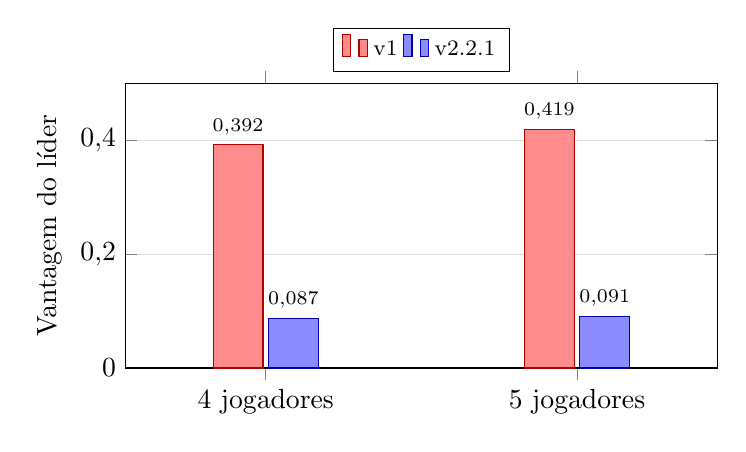
\begin{tikzpicture}
  \begin{axis}[
      ybar,
      bar width=18pt,
      width=0.75\linewidth,
      height=5.2cm,
      ymin=0, ymax=0.5,
      ylabel={Vantagem do líder},
      symbolic x coords={4 jogadores,5 jogadores},
      xtick=data,
      enlarge x limits=0.45,
      legend style={at={(0.5,1.04)}, anchor=south, legend columns=-1, font=\footnotesize},
      nodes near coords,
      every node near coord/.append style={font=\scriptsize, /pgf/number format/fixed,
        /pgf/number format/precision=3, /pgf/number format/use comma},
      yticklabel style={/pgf/number format/fixed, /pgf/number format/use comma},
      ymajorgrids=true,
      grid style={gray!25},
    ]
    \addplot[fill=red!45, draw=red!70!black] coordinates {(4 jogadores,0.392) (5 jogadores,0.419)};
    \addplot[fill=blue!45, draw=blue!70!black] coordinates {(4 jogadores,0.087) (5 jogadores,0.091)};
    \legend{v1, v2.2.1}
  \end{axis}
\end{tikzpicture}

  \caption{Vantagem do líder isolado após o ciclo 1 (chance de vencer menos $1/N$), na v1 e na v2.2.1}
  \label{fig:lider}
\end{figure}

\textbf{O melhor estilo é o Heurístico, que mistura construir e atacar.} A Tabela~\ref{tab:estilos} mostra a
taxa de vitória de um jogador de cada estilo (linha) numa mesa em que os outros três são de outro estilo
(coluna). O Heurístico é a melhor resposta, sozinho ou empatado, contra todas as mesas, menos a de Aleatórios. A
dinâmica do replicador termina em 100\% de Heurísticos, com 4 e com 5 jogadores. Nenhum Caçador puro é a melhor
resposta a mesa alguma, salvo a de Aleatórios: na v2.2.1, construir rende mais que caçar. Mesmo assim, os dois
estilos aparecem no jogo de quem joga bem. O Heurístico enche o sistema no 1º Planejamento em cerca de metade das
partidas e, nas outras, guarda cartas para testar (REQ-11). Habilidade importa: o Heurístico vence 0,938 das
partidas contra três Aleatórios, bem acima do piso de 0,375 (REQ-03).
% fonte: resultados/fase4_melhor_estilo/20261110-221516-ccd5649/relatorio.md

\begin{table}[ht]
  \centering
  \caption{Taxa de vitória do estilo da linha numa mesa com 3 jogadores do estilo da coluna (4 jogadores;
    referência 0,250; intervalos de cerca de $\pm 0{,}02$). Em negrito, as melhores respostas de cada coluna}
  \label{tab:estilos}
  \footnotesize
  \begin{tabular}{l c c c c c c}
    \toprule
    Estilo $\backslash$ Mesa & Aleatório & Construtor & Heurístico & Caç.\ líder & Caç.\ fraco & Caç.\ acaso \\
    \midrule
    Aleatório & 0,250 & 0,001 & 0,002 & 0,055 & 0,004 & 0,004 \\
    Construtor & \textbf{0,973} & \textbf{0,250} & \textbf{0,239} & \textbf{0,531} & 0,383 & \textbf{0,427} \\
    Heurístico & 0,938 & \textbf{0,264} & \textbf{0,250} & \textbf{0,549} & \textbf{0,434} & \textbf{0,451} \\
    Caçador (líder) & \textbf{0,965} & 0,168 & 0,113 & 0,250 & 0,387 & 0,294 \\
    Caçador (mais fraco) & 0,925 & 0,134 & 0,083 & 0,202 & 0,250 & 0,203 \\
    Caçador (ao acaso) & 0,943 & 0,146 & 0,087 & 0,234 & 0,325 & 0,250 \\
    \bottomrule
  \end{tabular}
\end{table}

\textbf{O blefe está equilibrado.} Num torneio entre 9 perfis puros de blefe (blefar nunca, metade das vezes ou
sempre; contestar nunca, sempre ou pelo limiar), nenhum perfil domina, e os perfis formam um ciclo. Blefar sempre
ganha de quem nunca contesta, contestar pelo limiar ganha de quem blefa, e não contestar ganha numa mesa de
honestos. O equilíbrio é uma mistura em que cerca de 1 em cada 6 jogadores blefa sempre. Nessa mistura, 39,5\% dos
blefes dão certo com 4 jogadores (intervalo de 38,6\% a 40,3\%) e 38,5\% com 5, dentro da faixa de 30\% a 50\% que
as regras pedem (REQ-05).
% fonte: resultados/fase4_exp5_blefe/20261110-231109-b02b6d4 e fase4_exp5b_blefe_equilibrio/20261111-004253-e17bbf2

\subsection{Requisitos, variantes e profundidade}

A Tabela~\ref{tab:resultados} resume os 13 requisitos, medidos com mesas de Heurísticos sorteadas do equilíbrio
do blefe, com conhecimento iniciante e experiente. Dez passam, dois passam em parte e um falha.

\begin{table}[ht]
  \centering
  \caption{Resultado dos requisitos na v2.2.1 (4 e 5 jogadores; iniciantes e experientes)}
  \label{tab:resultados}
  \footnotesize
  \begin{tabularx}{\linewidth}{>{\raggedright\arraybackslash}p{3.4cm} >{\raggedright\arraybackslash}p{1.6cm} >{\raggedright\arraybackslash}X}
    \toprule
    Requisito & Resultado & Valor medido \\
    \midrule
    REQ-01 Equidade de assento & em parte & Com bots aleatórios, todas as posições passam. Com Heurísticos, o 1º vence 0,276 e o último 0,224 (4 jogadores), na borda da zona \\
    REQ-02 Anti bola de neve & passa & 0,39 na v1 contra 0,09 na v2 \\
    REQ-03 Habilidade importa & passa & 0,938 (4 jog.) e 0,926 (5 jog.) \\
    REQ-04 Sem estratégia dominante & passa & Nenhum estilo nem perfil de blefe domina \\
    REQ-05 Blefes bem-sucedidos & passa & 0,395 e 0,385 \\
    REQ-06 Distribuição de ataques & passa & Razão de 1,35 a 1,43; fração contra o menor perto do limite com experientes \\
    REQ-07 Fichas não zeram cedo & passa & De 0,03 a 0,08 \\
    REQ-08 Duração & em parte & 44 min com 5 jogadores (passa); 38 min com 4 (abaixo de 40) \\
    REQ-09 Robustez & passa & 0 falhas em 971 mil partidas \\
    REQ-10 Tempo parado & \textbf{falha} & Percentil 90 de 5,8 min (4 jog.) e 9,0 min (5 jog.) \\
    REQ-11 Os dois estilos aparecem & passa & De 0,50 a 0,58 \\
    REQ-12 O 1º incidente não decide & passa & De 0,03 a 0,08 \\
    REQ-13 Incidentes pesam & passa & 0,29 (iniciantes) e 0,32 (experientes) \\
    \bottomrule
  \end{tabularx}
\end{table}

\textbf{Tempo e duração dependem de tempos ainda estimados.} Os tempos do modelo de duração são provisórios.
Com todos eles 25\% maiores, a partida de 4 jogadores passa a durar 48 minutos; com todos 25\% menores, o tempo
parado com 4 jogadores passa a 4,3 minutos. O resultado que não depende dos tempos é a relação entre os tamanhos de
mesa: a de 5 jogadores dura cerca de 15\% mais e fica cerca de 55\% mais tempo parada que a de 4. Por isso, a
v2.2.2 recomenda 4 jogadores (COR-03), mantendo o limite de 5.
% fonte: resultados/fase4_exp4_sensibilidade/20261111-082054-73762b5/relatorio.md

\textbf{O peso dos incidentes depende do conhecimento.} Medido só pelo dano, o peso dos incidentes era de 0,22
com iniciantes e de 0,17 com experientes, abaixo da zona. Quem sabe o conteúdo diagnostica melhor e se cobre
melhor, e por isso perde menos. Mas ganha mais no próprio incidente: pelos perfis do simulador, o experiente acerta o diagnóstico em 80\%
das vezes, e o iniciante em 40\%. Contando o incidente inteiro (dano e ganho do diagnóstico), o peso é de
0,29 com iniciantes e de 0,32 com experientes, e o requisito passa nos 40 cenários do Experimento 6. Essa
definição foi adotada pelo autor depois da primeira medição. A medida só pelo dano continua nos relatórios como
descrição.
% fonte: resultados/fase4_exp6_variantes/20261114-145900-0564baa/relatorio.md

\textbf{Nenhuma variante melhora tudo.} Das variantes propostas para o playtest:
\begin{itemize}
  \item comprar 2 cartas por Planejamento torna impossível encher o sistema no ciclo 1;
  \item cobrar uma ficha a mais pela explicação errada faz os iniciantes zerarem cedo;
  \item um Auditor externo, que não joga, piora o tempo parado;
  \item o vizinho designado e o limite de 2 testes recebidos encurtam a partida, mas concentram os ataques;
  \item a punição do blefe com 0 ou 2 fichas, o palpite da plateia e o módulo quase não mudam o que o simulador
    mede.
\end{itemize}
A regra atual foi a melhor das 10 configurações no conjunto. A ablação mostrou que cada mudança da 2.2, quando
desfeita, piora algum requisito ou não melhora nenhum. Com 6 jogadores (sem a COR-01), a mediana passa de 50
minutos, e o tempo parado chega a 12 minutos por ciclo. Com o bug duplicado permitido (regra da 2.1), os ataques
se concentram. Na sensibilidade, 5 fichas iniciais é o mínimo que passa no REQ-07: com 4 fichas, de 13\% a 23\% das
partidas têm alguém zerado antes do ciclo 3.
% fonte: fase4_exp6_variantes, fase4_exp3_ablacao/20261111-080955-f925943, fase4_exp4_sensibilidade, fase4_exp4b_combinacoes/20261111-134424-b263c34

\textbf{Testes sem limite dão o jogo mais profundo.} O Experimento 7 comparou a regra atual com 1 e 2 testes por
ciclo e com um custo de 1 ficha a partir do 2º teste do ciclo (Tabela~\ref{tab:profundidade}). Os testes sem
limite dão:
\begin{itemize}
  \item o maior número de decisões e de defesas por jogador;
  \item a menor vantagem do líder;
  \item a maior chance de recuperação de quem não lidera após o ciclo 1;
  \item o maior retorno para quem joga bem, medido pela vitória de um Heurístico normal contra Heurísticos mais
    descuidados (temperatura 4).
\end{itemize}
Com 1 teste por ciclo, a partida fica cerca de 10 minutos mais curta, mas é a regra mais rasa em todas as
medidas.
% fonte: resultados/fase4_exp7_profundidade/20261111-183119-3a2f2e0/relatorio.md

\begin{table}[ht]
  \centering
  \caption{Profundidade das regras de teste. Duração mediana em minutos com 4 e 5 jogadores; defesas e decisões
    por jogador; vantagem do líder (faixa entre iniciantes e experientes); ``jogar bem'': vitória do jogador
    cuidadoso dividida por $1/N$ contra jogadores descuidados, com 4 e 5 jogadores}
  \label{tab:profundidade}
  \footnotesize
  \setlength{\tabcolsep}{4pt}
  \begin{tabular}{l c c c c c}
    \toprule
    Regra & Duração & Defesas & Decisões & Vantagem do líder & Jogar bem \\
    \midrule
    \textbf{Sem limite (atual)} & 38 / 44 & \textbf{5,5} & \textbf{33} & \textbf{0,15--0,19} & \textbf{1,88 / 2,10} \\
    Custo a partir do 2º teste & 34 / 39 & 4,1 & 30 & 0,18--0,22 & 1,86 / 2,10 \\
    2 testes por ciclo & 33 / 38 & 4,0 & 28 & 0,18--0,21 & 1,68 / 1,92 \\
    1 teste por ciclo & 28 / 32 & 2,2 & 22 & 0,22--0,27 & 1,60 / 1,78 \\
    \bottomrule
  \end{tabular}
\end{table}

\subsection{QP2: como os estudantes avaliam a experiência?}

Responderam ao questionário 7 estudantes de três cursos: 4 de Ciência da Computação, 2 de Ciência de Dados e
Inteligência Artificial e 1 de Engenharia da Computação. Todos estavam do 6º período em diante. Dois tinham
experiência profissional com teste. Quatro avaliaram o próprio conhecimento prévio sobre testes não funcionais
com 4 numa escala de 5. A Tabela~\ref{tab:playtest} mostra as respostas às afirmações.

\begin{table}[ht]
  \centering
  \caption{Respostas ao questionário do playtest (7 respondentes; DT: discordo totalmente; D: discordo; N: nem
    concordo nem discordo; C: concordo; CT: concordo totalmente)}
  \label{tab:playtest}
  \scriptsize
  \begin{tabularx}{\linewidth}{>{\raggedright\arraybackslash}X c c c c c c}
    \toprule
    Afirmação & DT & D & N & C & CT & C+CT \\
    \midrule
    \multicolumn{7}{l}{\textit{Sobre o jogo}} \\
    O design do jogo é atraente & 0 & 0 & 1 & 2 & 4 & 6/7 \\
    Aprender a jogar este jogo foi fácil & 0 & 0 & 2 & 2 & 3 & 5/7 \\
    As regras do jogo são claras e compreensíveis & 0 & 0 & 1 & 5 & 1 & 6/7 \\
    Este jogo é adequadamente desafiador & 0 & 0 & 3 & 3 & 1 & 4/7 \\
    Me sinto satisfeito com o que aprendi no jogo & 0 & 1 & 1 & 1 & 4 & 5/7 \\
    Eu recomendaria este jogo para meus colegas & 1 & 0 & 2 & 1 & 3 & 4/7 \\
    O jogo promove cooperação e/ou competição & 0 & 0 & 1 & 1 & 5 & 6/7 \\
    Eu me diverti com o jogo & 0 & 0 & 1 & 1 & 5 & 6/7 \\
    Eu estava tão envolvido que perdi a noção do tempo & 0 & 0 & 1 & 1 & 5 & 6/7 \\
    É claro como o conteúdo se relaciona com a disciplina & 0 & 0 & 2 & 1 & 4 & 5/7 \\
    O jogo contribuiu para a minha aprendizagem na disciplina & 0 & 1 & 1 & 1 & 4 & 5/7 \\
    \midrule
    \multicolumn{7}{l}{\textit{O jogo contribuiu para eu\ldots}} \\
    \ldots lembrar os tipos de teste de cada categoria & 0 & 0 & 3 & 3 & 1 & 4/7 \\
    \ldots explicar com minhas palavras o que um teste verifica & 0 & 1 & 2 & 3 & 1 & 4/7 \\
    \ldots identificar a característica afetada numa falha real & 0 & 0 & 2 & 3 & 2 & 5/7 \\
    \ldots decidir quais testes priorizar pelo contexto e pelo risco & 0 & 0 & 2 & 2 & 3 & 5/7 \\
    \midrule
    \multicolumn{7}{l}{\textit{Sobre as regras}} \\
    Acompanhar a pontuação com as fichas foi fácil & 0 & 0 & 3 & 0 & 4 & 4/7 \\
    Explicar o teste com minhas palavras me fez pensar no conteúdo & 0 & 0 & 3 & 2 & 2 & 4/7 \\
    O Radar me ajudou a decidir quais testes colocar no sistema & 0 & 0 & 4 & 1 & 2 & 3/7 \\
    Senti que fui testado muito mais vezes que os outros & 1 & 1 & 2 & 2 & 1 & 3/7 \\
    Até perto do fim, eu achava que ainda podia vencer & 1 & 0 & 2 & 3 & 1 & 4/7 \\
    Decidir entre colocar a carta no sistema ou testar foi interessante & 0 & 0 & 1 & 2 & 4 & 6/7 \\
    \bottomrule
  \end{tabularx}
\end{table}
% fonte: uv run python scripts/resumir_playtest.py (CSV local, fora do git)

Os sete respondentes marcaram que se divertiram jogando. Cinco disseram que o jogo serviu como revisão de
conteúdos que já tinham estudado, três que aprenderam conceitos novos e dois que perceberam que precisam estudar
mais o tema. Para a duração, 5 responderam ``adequada'' e 2, ``longa demais''. A parte mais confusa foi a
Homologação, com o blefe e a contestação, para 4 respondentes, e a pontuação com fichas para 2. Entre os pontos
fortes, os respondentes citaram a diversão, o blefe, as ilustrações e a relação entre as categorias de teste e
situações práticas. Entre as mudanças sugeridas, dois pediram para punir mais o blefe, um pediu para simplificar
a pontuação das disputas, um sugeriu uma área de jogo para organizar cartas e fichas, e um sugeriu simplificar o
jogo.

As respostas conversam com o simulador em quatro pontos:
\begin{itemize}
  \item \textbf{A decisão central foi percebida.} A afirmação com mais concordância entre as de regras, ``decidir
    entre colocar a carta no sistema ou testar foi interessante'' (6 de 7), é justamente a decisão que o
    Experimento~7 aponta como a fonte da profundidade do jogo.
  \item \textbf{O blefe pareceu impune para os jogadores, mas não para os bots.} No simulador, o blefe está
    equilibrado: quem contesta pelo limiar pega quase todo blefe, e mudar a punição para 0 ou 2 fichas quase não
    altera os requisitos. A diferença provável está na contestação. Os bots contam as cartas já vistas e sabem
    quando um teste nomeado está esgotado, e pessoas contam pior e talvez contestem menos. O próximo playtest deve
    registrar quantas contestações acontecem.
  \item \textbf{A sensação de ser testado demais} (3 de 7 concordam) contrasta com o REQ-06, que passa no
    simulador. Com poucas partidas, a variação de uma partida para outra pode explicar a impressão.
  \item \textbf{O Radar} foi o elemento com menor concordância (3 de 7). Nos bots, a leitura do Radar orienta a
    construção do sistema, mas os estudantes podem não ter percebido essa função.
\end{itemize}

Comparando com a v1, em que 14 de 17 respondentes disseram ter se divertido e 9 que o jogo serviu como revisão
\cite{oliveira2025critical}, as proporções na v2 são parecidas ou maiores (7 de 7 e 5 de 7). As amostras e os
questionários são diferentes, e a comparação é só descritiva.

\subsection{Balanceamento como teste não funcional}

O artigo da v1 apontou paralelos entre projetar um jogo e testar requisitos não funcionais, como usabilidade,
robustez e acessibilidade \cite{oliveira2025critical}. Este trabalho levou o paralelo adiante e tratou o
balanceamento como um requisito não funcional verificável. Algumas lições:
\begin{itemize}
  \item \textbf{Critério antes do resultado.} Fixar a medida e a zona de aceite antes de medir evitou que o
    critério se ajustasse ao resultado. Quando o critério mudou depois da medição, como no REQ-13, a mudança
    foi registrada e as duas leituras foram mantidas.
  \item \textbf{O problema do oráculo.} Não há um valor esperado para ``jogo balanceado''. Relações
    metamórficas, como trocar o nome das categorias sem mudar as partidas, e invariantes, como a conservação das
    cartas, serviram de oráculos parciais \cite{chen1998,segura2016}.
  \item \textbf{Os testes do simulador acharam defeitos reais.} O fuzzing achou uma brecha na auditoria: o
    \texttt{replay} não conferia a linha final inteira, e um registro adulterado passava. O teste de mutação
    apontou regras e medidas sem teste, e as invariantes nunca eram testadas com estados inválidos. Todas essas
    lacunas foram fechadas com testes novos.
  \item \textbf{Determinismo como evidência.} O Experimento 6 foi repetido três dias depois, com outro número
    de processos e muitos commits no meio, e as 80 mil partidas saíram idênticas. Isso dá confiança de que cada
    número pode ser refeito.
  \item \textbf{Ablação como teste de regressão do projeto.} Desfazer cada mudança de regra e medir de novo
    mostrou quais decisões de projeto se sustentam nos dados.
\end{itemize}

\subsection{Limitações e ameaças à validade}

Seguindo Wohlin et al. \cite{wohlin2012}, destacam-se as seguintes ameaças:
\begin{itemize}
  \item \textbf{Bots não são estudantes.} O simulador mede o balanceamento da mecânica, não a aprendizagem nem a
    diversão. Os perfis de conhecimento indicam se a mecânica se degrada com pouco conhecimento, mas não
    representam um estudante real. Os bots também contam cartas melhor que pessoas.
  \item \textbf{Os estilos foram escritos à mão.} ``Nenhum estilo dominante'' vale entre os seis estilos
    implementados. O REQ-04 de estilos passou só por causa da mesa de Aleatórios.
  \item \textbf{Os tempos são estimados.} Os vereditos de duração e de tempo parado só valem de fato com os
    tempos cronometrados em partidas reais.
  \item \textbf{Um critério mudou depois da medição.} A definição do REQ-13 passou a contar o diagnóstico depois
    de o requisito falhar com experientes, por decisão do autor. As duas leituras são relatadas.
  \item \textbf{A v1 foi validada com poucas partidas.} O simulador reproduz o mecanismo da bola de neve, mas a
    referência do artigo são 6 partidas.
  \item \textbf{O playtest é pequeno.} Foram 7 respostas de cerca de 30 participantes, uma delas com ``nem
    concordo nem discordo'' em todos os itens. As respostas são autoavaliações e dizem respeito à v2.2 com o
    módulo, anterior às correções da v2.2.1 e da v2.2.2. Os resultados não podem ser generalizados.
\end{itemize}

\section{Conclusões e Trabalhos Futuros}
\label{sec:conclusoes}

Este trabalho redesenhou as regras do Critical Failure e verificou o seu balanceamento com um simulador
determinístico e auditável, que tratou o jogo como um sistema sob teste. O balanceamento virou um conjunto de 13
requisitos não funcionais com critério de aceite, verificados em 971 mil partidas entre bots com estilos de jogo
diferentes.

Quanto à \textbf{QP1}, as novas regras reduzem o desequilíbrio da primeira versão. Com os mesmos bots e as mesmas
sementes, a vantagem de quem lidera após o primeiro ciclo cai de cerca de 0,40 para cerca de 0,09, e atacar o
líder passa a compensar. A v2 passa em 10 dos 13 requisitos, entre eles a ausência de estratégia dominante, o
equilíbrio do blefe e o peso dos incidentes. O melhor estilo é o que mistura construir e atacar conforme o valor
de cada jogada. Os pontos fracos são o tempo parado, sobretudo com 5 jogadores, a duração com 4 jogadores e uma
pequena vantagem do primeiro jogador entre bots que jogam bem. Os dois primeiros dependem dos tempos reais das
ações. A versão atual (v2.2.2) recomenda 4 jogadores, e os testes sem limite, que dão o jogo mais profundo, foram
mantidos.

Quanto à \textbf{QP2}, os 7 estudantes que responderam ao questionário avaliaram o jogo de forma positiva: todos
marcaram que se divertiram, e a maioria viu relação clara com a disciplina e contribuição para a aprendizagem. A
Homologação, com o blefe e a contestação, foi a parte mais confusa, e houve pedidos para punir mais o blefe. Pelo
tamanho da amostra, esses resultados são indícios, não conclusões.

Como trabalhos futuros, propõem-se:
\begin{itemize}
  \item um novo playtest com a v2.2.2, com as ações cronometradas, para substituir os tempos do modelo de duração
    e julgar de fato a duração e o tempo parado, e com o registro de cada contestação;
  \item a avaliação com o questionário completo do MEEGA+ \cite{petri2017meega} numa turma maior;
  \item a calibração dos perfis de conhecimento dos bots com os dados das folhas de registro das partidas reais;
  \item uma busca automática de estratégias, por exemplo evolutiva, para verificar se existe um estilo que
    domine todos os outros além dos seis escritos à mão.
\end{itemize}

\section*{Disponibilidade dos artefatos}

O simulador, as regras de cada versão em texto, as configurações, os experimentos e, para cada execução
oficial, o manifesto e o relatório estão disponíveis em \pendente{link público do repositório}. As tabelas de
partidas e os registros de auditoria podem ser refeitos a partir dos manifestos.

As respostas individuais ao questionário do playtest não são publicadas, para proteger a privacidade dos
participantes, como no artigo da primeira versão \cite{oliveira2025critical}. Este texto traz apenas contagens
agregadas.

\section*{Uso de inteligência artificial}

As imagens das cartas foram geradas com o GPT 6. Um assistente de inteligência artificial foi usado no
desenvolvimento do código do simulador e na redação de uma versão preliminar deste texto. As decisões sobre as
regras, os parâmetros, os critérios de aceite e a interpretação dos resultados foram do autor e estão registradas
no diário de bordo do repositório.


\bibliographystyle{sbc}
\bibliography{referencias}

\end{document}
